\documentclass{article}

\usepackage[utf8]{inputenc}
\usepackage[russian]{babel}
\usepackage{amsmath}
\usepackage{amssymb}
\usepackage{graphicx}
\usepackage{hyperref}

\newcommand{\myparagraph}[1]{\paragraph{#1}\mbox{}\\}

\title{Homework 7}
\date{2018-27-10}
\author{Dimitrov Blagoi}

\begin{document}
  \pagenumbering{gobble}
  \maketitle
  \newpage
  \pagenumbering{arabic}

  \newpage

  \myparagraph{Задание 1}
  Пример СС для 5 нитей с 9-ю компараторами:

  \begin{figure}[h!]
    \centering
    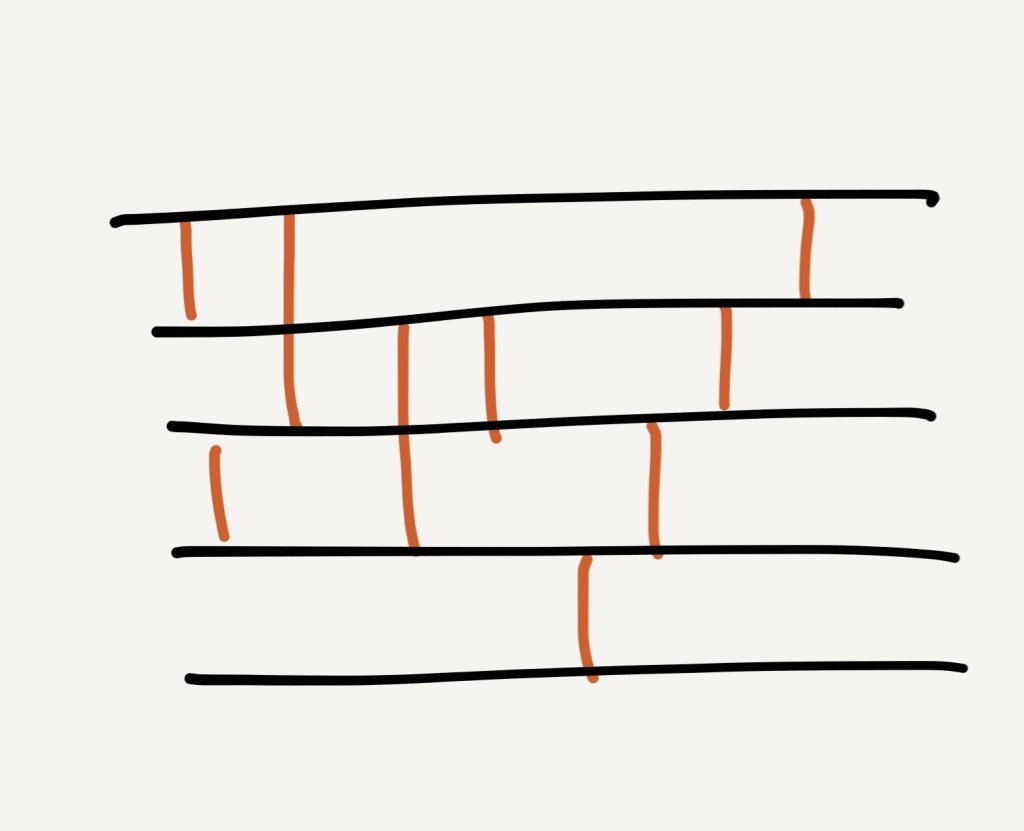
\includegraphics[width = 0.8\linewidth]{Pictures/Picture1.jpg}
  \end{figure}

  Очевидно, что эта сеть сортирующая. (я перебрал все варианты).

  Меньше очевидно нельзя, по теореме о минимальном колличестве компараторов в сортирующих сетях.

  \begin{flushright}
    $\blacksquare$
  \end{flushright}

  \newpage

  \myparagraph{Задание 2}
  \begin{figure}[h!]
    \centering
    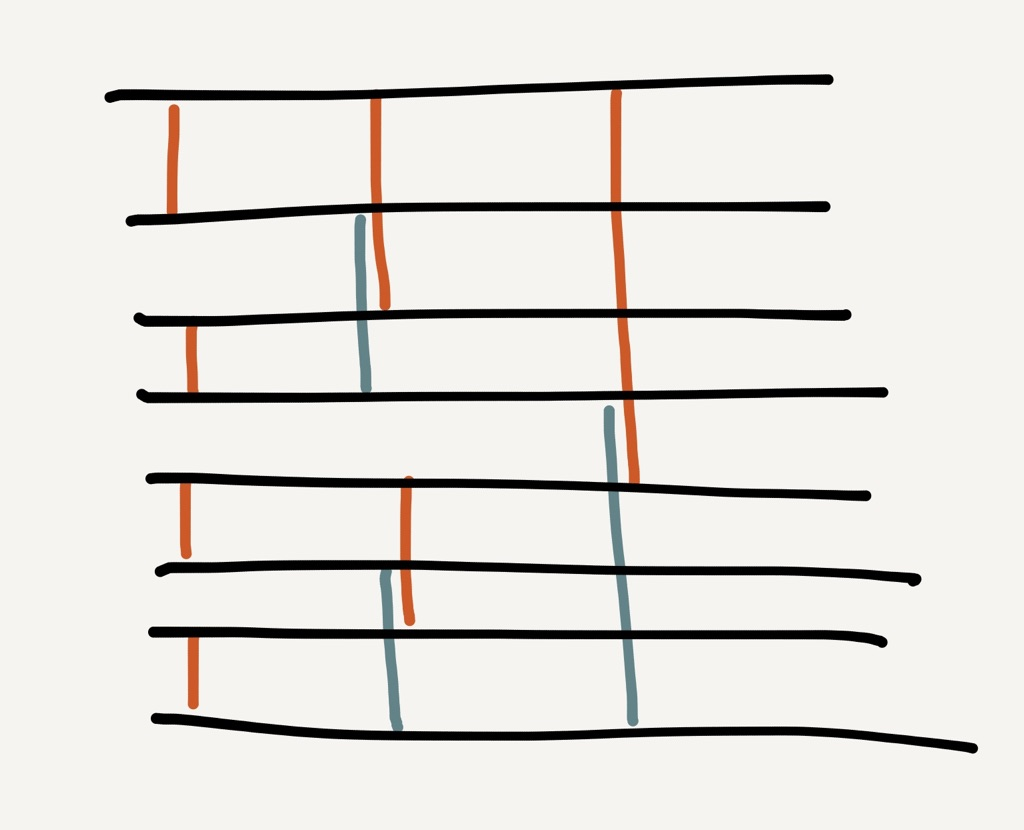
\includegraphics[width = 0.8\linewidth]{Pictures/Picture2.jpg}
  \end{figure}

  Очевидно, что данная сеть ставит на нижнюю ветку максимальное число, на верхнюю - минимальное. Где бы не стоял минимальный элемент, на кажлом шаге он будет проталкиваться красными компараторами наверх и в конце концов попадет наверх. Аналогично максимум. Глубина лог по построению. (синие и красные компараторы могут выполнять сравнения параллельно, т.к. сравнивают разные элементы.)

  \begin{flushright}
    $\blacksquare$
  \end{flushright}


 \end{document}